\documentclass{article}

\usepackage[submission]{colm2026_conference}
\usepackage{microtype}
\usepackage{hyperref}
\usepackage{url}
\usepackage{booktabs}
\usepackage{graphicx}
\usepackage{amsmath}
\usepackage{amssymb}
\usepackage{tikz}
\usepackage{lineno}

\definecolor{darkblue}{rgb}{0, 0, 0.5}
\hypersetup{colorlinks=true, citecolor=darkblue, linkcolor=darkblue, urlcolor=darkblue}

\title{Ask, Don't Guess: Learning When to Clarify in Situated Instruction Following}

\begin{document}

\ifcolmsubmission
\linenumbers
\fi

\maketitle

\begin{abstract}
Language agents deployed in situated environments must decide not only what an instruction might mean, but whether it is useful to act on that interpretation. Existing ambiguity and clarification evaluations often frame this as a static language-understanding problem: detect ambiguity and ask a question. We argue that clarification is instead a situated decision under uncertainty, interaction cost, and task consequences. We introduce \textsc{Clarify-to-Act}, a procedurally generated benchmark in which an agent receives a structured scene and a user instruction, then must either act immediately or ask one clarifying question before acting. The environment provides deterministic rewards based on final task success minus clarification cost, enabling cheap learning from interaction without human labels or model weight updates. In a 100-episode stratified API evaluation with GPT-4.1-mini, a prompted ask-when-needed baseline reaches 0.632 net utility and misses 58.3\% of oracle clarification cases, while an expected-communicative-utility policy reaches 0.976 net utility with 100\% task success and no missed or unnecessary clarifications.
\end{abstract}

\section{Introduction}

Situated language agents frequently face instructions that are underspecified relative to the action space. A household assistant asked to ``bring the red mug'' may see two red mugs. A file-management agent asked to ``delete the old draft'' may see two plausible drafts with very different consequences. In these cases, the agent must decide whether to act immediately or ask a clarifying question.

The usual framing asks whether the user query is ambiguous \citep{zhang2024clamber,kuhn2022clam}. That framing is incomplete. Some ambiguous instructions are resolved by the environment: if only one cup is reachable on the active workspace, asking wastes interaction. Some underspecified instructions are harmless because all choices are equivalent: ``move a spare chair to the table'' does not require identifying a particular spare chair. Other cases are high risk: even a likely interpretation of ``delete the old file'' may warrant clarification if the wrong action is costly.

We study clarification as a situated decision problem. The relevant question is not simply whether language admits multiple interpretations, but whether the expected value of clarification exceeds its interaction cost. This connects clarification to situated instruction following \citep{min2024situated} and value-of-information views of questions \citep{rao2018learning}, while keeping the benchmark lightweight and deterministic.

This paper makes three contributions. First, we introduce \textsc{Clarify-to-Act}, a procedural benchmark for ask-or-act decisions in structured scenes. Second, we define an expected communicative utility objective that provides automatic oracle labels and task-level net utility. Third, we evaluate deterministic baselines, a lightweight learned controller, and API-based language-agent policies. Expected-utility calibration improves net utility by reducing both guessing and unnecessary clarification.

\section{Clarify-to-Act}

Each episode contains a scene, a user instruction, candidate intents, a hidden user intent, a simulated user, and a deterministic reward. The agent observes the scene and instruction and outputs either:
\[
\{\texttt{type}:\texttt{ACT},\ \texttt{action}:a,\ \texttt{target\_id}:o\}
\]
or:
\[
\{\texttt{type}:\texttt{ASK},\ \texttt{question}:q\}.
\]
If it asks, the simulated user returns one answer from the hidden intent and the agent must then act. Episodes are at most two turns.

\begin{figure}[t]
\centering
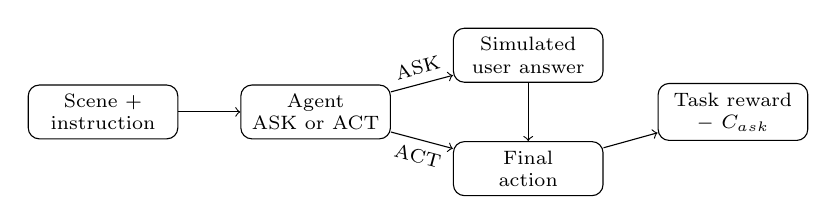
\begin{tikzpicture}[font=\scriptsize, x=1cm, y=1cm]
  \node[draw, rounded corners, align=center, minimum width=1.9cm, minimum height=0.62cm] (input) at (0,0) {Scene +\\instruction};
  \node[draw, rounded corners, align=center, minimum width=1.9cm, minimum height=0.62cm] (agent) at (2.7,0) {Agent\\ASK or ACT};
  \node[draw, rounded corners, align=center, minimum width=1.9cm, minimum height=0.62cm] (act) at (5.4,-0.72) {Final\\action};
  \node[draw, rounded corners, align=center, minimum width=1.9cm, minimum height=0.62cm] (answer) at (5.4,0.72) {Simulated\\user answer};
  \node[draw, rounded corners, align=center, minimum width=1.9cm, minimum height=0.62cm] (reward) at (8.0,0) {Task reward\\$-\ C_{ask}$};
  \draw[->] (input) -- (agent);
  \draw[->] (agent) -- node[above, sloped] {ASK} (answer);
  \draw[->] (answer) -- (act);
  \draw[->] (agent) -- node[below, sloped] {ACT} (act);
  \draw[->] (act) -- (reward);
\end{tikzpicture}
\caption{\textsc{Clarify-to-Act} interaction protocol. The agent either acts immediately or asks one clarifying question, then receives deterministic task reward minus interaction cost.}
\label{fig:task-overview}
\end{figure}

\begin{table}[t]
\centering
\scriptsize
\begin{tabular}{@{}p{0.17\linewidth}p{0.22\linewidth}c p{0.37\linewidth}@{}}
\toprule
Category & Example instruction & Oracle ask & Diagnostic contrast \\
\midrule
Referential & Bring the black box & 1.00 & Matching objects, wrong target matters \\
Context-resolved & Pass the folder I'm using & 0.00 & Context or salience resolves intent \\
Equivalent outcome & Move a spare folder & 0.00 & Any target in success class works \\
Risk-sensitive & Delete the old draft & 1.00 & Wrong action has high cost \\
Preference/social & Put my cup away & 0.50 & Owner visible vs. hidden \\
\bottomrule
\end{tabular}
\caption{Benchmark categories. Each category has 280 episodes in the canonical dataset; the oracle ask rate follows expected communicative utility.}
\label{tab:benchmark-categories}
\end{table}

\paragraph{Diagnostic categories.}
Table~\ref{tab:benchmark-categories} summarizes the five diagnostic categories. The current dataset contains 1,400 episodes: 600 train, 200 dev, 400 test, and 200 OOD test episodes. Splits are balanced across categories and the overall oracle ask rate is 0.50.

\paragraph{Reward and oracle.}
The reward is
\[
R = \mathbb{1}[\mathrm{success}] - C_{ask}\mathbb{1}[\mathrm{asked}] - C_{wrong}\mathbb{1}[\mathrm{wrong}].
\]
Success is defined by matching the hidden intent's success-equivalence class, so interchangeable actions can succeed without arbitrary target identity matches. Let $p_{\max}$ be the probability mass of the best success-equivalence class. We compute
\[
EU(act) = p_{\max} - (1-p_{\max})C_{wrong}, \qquad EU(ask)=1-C_{ask}.
\]
The oracle asks when $EU(ask) > EU(act)+\epsilon$.

\paragraph{Leakage controls.}
API smoke tests exposed possible leakage in the preference/social category. The final benchmark uses neutral target IDs, redacts hidden object owners from API prompts, gives hidden-owner objects neutral state labels, and includes \texttt{current\_user} only as user identity. Visible-owner cases remain resolvable; hidden-owner cases require clarification.

\section{Methods}

\paragraph{DirectAct.}
The agent acts immediately and never asks.

\paragraph{AskAlways and raw ambiguity.}
AskAlways always asks before acting. Raw ambiguity asks whenever more than one candidate target exists.

\paragraph{Prompted Ask-Needed.}
An API language model receives a prompt instructing it to ask only when acting could plausibly fail. This is the strongest simple prompting baseline and is related to recent language-agent clarification work \citep{qian2024tell}.

\paragraph{Expected communicative utility.}
The ECU policy asks the model to propose candidate interpretations with probabilities and metadata. Python computes expected utility from the candidates, ask cost, and wrong-action cost. If the margin favors asking, the model generates one clarifying question; otherwise the agent acts on the best candidate. The final API ECU policy uses an ask margin of 0.075, visibility redaction for hidden-owner cases, and a conservative equivalence guard so the model can only collapse candidates into one success class when the instruction contains equivalence cues such as ``spare'' or ``any.''

\paragraph{Learned controller.}
The offline learned controller is a lightweight logistic ask/act model trained from automatic oracle labels. It uses features such as number of candidates, number of success classes, top prior, entropy, ask cost, wrong-action cost, salience gap, risk, context resolution, equivalence, and expected-utility margin.

\begin{table}[t]
\centering
\scriptsize
\begin{tabular}{@{}lll@{}}
\toprule
Method & Ask/act signal & Diagnostic role \\
\midrule
DirectAct & Never asks & Guessing under ambiguity and risk \\
AskAlways / raw ambiguity & Always ask / target count & Over-clarification and ambiguity-only behavior \\
Prompted Ask-Needed & Ask-or-act prompt & Strong simple prompting baseline \\
CoT Ask-Needed & Private-reasoning prompt & Reasoning-only calibration test \\
API ECU & Model candidates + expected utility & Main utility-calibrated policy \\
Threshold / controller & Tuned margin / logistic model & Interaction-supervised calibration \\
\bottomrule
\end{tabular}
\caption{Method summary. The key comparison is not only whether a method detects ambiguity, but whether its ask/act decision is calibrated to expected task utility.}
\label{tab:methods}
\end{table}

\section{Experiments}

We report offline benchmark evaluation, API evaluation, and cost sensitivity. Offline evaluation uses the full 400-episode test split and 200-episode OOD split. API evaluation uses GPT-4.1-mini on a 100-episode stratified subset with 20 episodes per category. We additionally construct a 50-episode stress set by paraphrasing test instructions and shifting simulated user answers to terser location/owner-style replies. As a small model-coverage sanity check, we also run GPT-4.1-nano on 25 stratified test episodes. Calls are cached; the final main cache contains 914 responses, 271,208 input tokens, and 49,117 output tokens.

\paragraph{Reproducibility.}
The artifact package includes a generated reproducibility report with dataset and result hashes, recomputed metrics, API cache token totals, and exact commands. It also includes automated claim-verification and simulated-user answer audits. The final API evaluation can be replayed in cache-only mode, which fails on any cache miss rather than making a network call.

\begin{figure}[t]
\centering
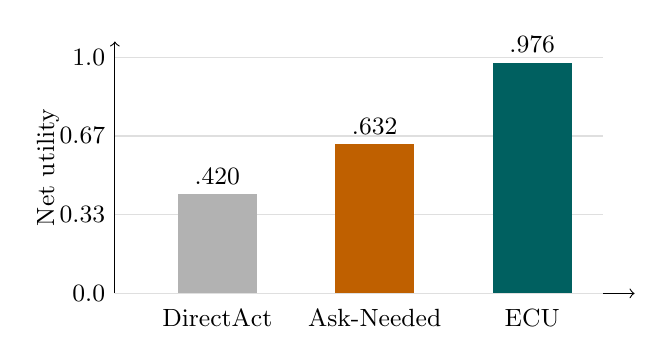
\begin{tikzpicture}[x=1cm,y=1cm]
  \draw[->] (0,0) -- (6.6,0);
  \draw[->] (0,0) -- (0,3.2);
  \foreach \y/\lab in {0/0.0,1/0.33,2/0.67,3/1.0} {
    \draw[gray!25] (0,\y) -- (6.2,\y);
    \node[left] at (0,\y) {\small \lab};
  }
  \fill[gray!60] (0.8,0) rectangle (1.8,1.26);
  \fill[orange!75!black] (2.8,0) rectangle (3.8,1.90);
  \fill[teal!75!black] (4.8,0) rectangle (5.8,2.93);
  \node[below] at (1.3,-0.08) {\small DirectAct};
  \node[below] at (3.3,-0.08) {\small Ask-Needed};
  \node[below] at (5.3,-0.08) {\small ECU};
  \node[above] at (1.3,1.26) {\small .420};
  \node[above] at (3.3,1.90) {\small .632};
  \node[above] at (5.3,2.93) {\small .976};
  \node[rotate=90] at (-0.85,1.6) {\small Net utility};
\end{tikzpicture}
\caption{Main API result on 100 stratified test episodes. ECU substantially improves net utility over direct action and prompted ask-when-needed.}
\label{fig:api-main}
\end{figure}

\begin{table}[t]
\centering
\small
\begin{tabular}{lrrrrrr}
\toprule
Method & $N$ & Utility & Success & Ask & Missed & Unnec. \\
\midrule
DirectAct & 100 & 0.420 & 0.770 & 0.000 & 1.000 & 0.000 \\
Ask-Needed & 100 & 0.632 & 0.880 & 0.370 & 0.583 & 0.327 \\
API ECU & 100 & 0.976 & 1.000 & 0.480 & 0.000 & 0.000 \\
\bottomrule
\end{tabular}
\caption{API evaluation with GPT-4.1-mini. Utility is the primary metric.}
\label{tab:api-main}
\end{table}

\section{Results}

Table~\ref{tab:api-main} and Figure~\ref{fig:api-main} show the main API result. DirectAct fails because it never asks, producing low success in referential and risk-sensitive cases. Prompted Ask-Needed improves over DirectAct but remains poorly calibrated: it misses 58.3\% of oracle clarification cases and asks unnecessarily in 32.7\% of oracle-act cases. A private-reasoning variant of Ask-Needed does not improve net utility (0.632) and still misses 60.4\% of oracle clarification cases. API ECU reaches 0.976 net utility and 100\% success, with no missed or unnecessary clarifications in this stratified evaluation. Because all policies run on the same episodes, paired bootstrap deltas are the appropriate comparison: ECU exceeds Ask-Needed by 0.343 net utility with 95\% paired CI [0.168, 0.559], and exceeds the private-reasoning variant by 0.344 [0.171, 0.564].
Conditional on asking, both Ask-Needed and ECU successfully ground the simulated answer in the main set; the gap is ask timing. ECU has ask precision/recall/post-answer success of 1.000/1.000/1.000, while Ask-Needed has 0.541/0.417/1.000.

\begin{table}[t]
\centering
\small
\begin{tabular}{lrrrrr}
\toprule
Category & Direct & Ask-Needed & ECU & ECU Ask & Oracle Ask \\
\midrule
Context-resolved & 1.000 & 0.993 & 1.000 & 0.000 & 0.000 \\
Preference/social & 0.400 & 0.400 & 0.980 & 0.400 & 0.400 \\
Equivalent-outcome & 1.000 & 0.920 & 1.000 & 0.000 & 0.000 \\
Referential & -0.100 & 0.857 & 0.950 & 1.000 & 1.000 \\
Risk-sensitive & -0.200 & -0.008 & 0.950 & 1.000 & 1.000 \\
\bottomrule
\end{tabular}
\caption{API net utility by category. ECU asks when clarification matters and avoids asking when context or outcome equivalence resolves the instruction.}
\label{tab:api-category}
\end{table}

Table~\ref{tab:api-category} shows that the ECU advantage is not driven by a single category. Prompted Ask-Needed performs well on referential ambiguity but over-asks equivalent-outcome cases and misses most risk-sensitive cases. ECU asks in all referential and risk-sensitive cases, avoids all context-resolved and equivalent-outcome cases, and matches the oracle ask rate in preference/social cases.
In a no-API subset-stability diagnostic, ECU--Ask-Needed remains positive after omitting any one category (minimum +0.190) or any one episode (minimum +0.307), and a category-stratified bootstrap gives 95\% CI [0.183, 0.541].

\paragraph{Ambiguity is not enough.}
A no-API diagnostic isolates the central distinction from raw ambiguity detection. All 400 canonical test episodes have multiple candidate interpretations, but exactly 200 are oracle-act cases and 200 are oracle-ask cases. A surface-ambiguity policy therefore asks on every episode, reaching 0.920 utility with unnecessary clarification rate 1.000. A supervised uncertainty-only controller trained only on candidate count, top prior, and prior entropy reaches 0.900 utility, but still misses 7.0\% of oracle-ask cases and asks unnecessarily in 40.0\% of oracle-act cases. ECU and the full learned controller reach 0.958 utility while eliminating both missed and unnecessary clarification on the same offline test split.
A situated contrast diagnostic makes the same point at the slice level. Among two-candidate \texttt{bring} episodes, all 80 context-resolved cases are oracle-act while all 80 referential cases are oracle-ask. For \texttt{put\_away} preference episodes, visible ownership gives oracle-act on 40/40 cases, while hidden ownership gives oracle-ask on 40/40. High-entropy equivalent-outcome cases are oracle-act because all candidates share one success class, whereas high-top-prior risk-sensitive cases are oracle-ask because the wrong-action cost is high.

\paragraph{Utility-margin calibration.}
We also bin episodes by the oracle expected-utility margin $EU(ask)-EU(act)$. On the main API set, ECU asks on 0/40 act-preferred episodes and 48/48 ask-preferred episodes. Prompted Ask-Needed asks on 17/40 act-preferred episodes and only 20/48 ask-preferred episodes. On the paraphrase/style stress set, ECU again asks on 0/20 act-preferred and 23/23 ask-preferred episodes, while Ask-Needed asks on 7/20 and 12/23. Thus the prompted baseline is not calibrated to value of information: it asks at similar rates when asking is harmful and when asking is useful.
As an internal cached-row diagnostic, API ECU's model-derived candidate-margin threshold agrees with the oracle ask label on 99/100 main API rows; after the effective context override, final ask/oracle agreement is 100/100. This supports that the API-side candidate scoring is aligned on the evaluated subset, but it is not an independent benchmark.

A cached decision ablation isolates the role of the equivalence guard. Replaying the same model candidate interpretations, accepting every model-declared equivalence flag drops utility to 0.745 and misses 37.5\% of oracle-ask cases. Never collapsing equivalent candidates keeps success at 100\% but raises unnecessary clarification to 38.5\%. The conservative guard is therefore needed in both directions: it prevents unsafe over-collapsing in true ambiguity while still allowing action in equivalent-outcome cases.

On the full 400-episode offline test set, ECU and the learned controller reach 0.958 net utility, compared with 0.938 for the prompted heuristic, 0.920 for AskAlways, and 0.498 for DirectAct. On the 200-episode OOD split, ECU reaches 0.975 utility versus 0.955 for the prompted heuristic. The OOD split preserves all five diagnostic categories and shifts object types where supported by the generator; 102 OOD episodes contain at least one held-out object type. On this held-out-object slice, ECU and the learned controller reach 0.975 utility and 100\% success, while keeping ask rate at 0.500. The learned controller is interpretable: its largest positive weights are expected-utility margin, risk, and entropy, while context resolution, equivalence, and ask cost push toward acting.

We also run a no-API held-out ambiguity-mix diagnostic. Train/dev/test episodes contain only referential, context-resolved, and equivalent-outcome cases; the held-out split contains risk-sensitive and preference/social cases. ECU transfers with 0.962 held-out utility, nearly unchanged from 0.963 on the seen-category test split. The tuned threshold and learned controller reach 0.950 but ask on all held-out episodes, over-clarifying visible preference/social cases. This is a useful boundary on the learning claim: the controller is transparent and effective when the diagnostic categories are represented, while the expected-utility rule is more stable under this category shift.

As an external query-level sanity check, we map CLAMBER's \texttt{require\_clarification} field to an ASK label \citep{zhang2024clamber}. The benchmark's provided \texttt{predict\_ambiguous} field has 0.284 recall and 0.716 missed-clarification rate against that label. This is not a situated task-utility result, but it supports the motivation that ambiguity prediction alone can under-identify clarification needs.

\paragraph{Paraphrase and answer-style stress.}
On the 50-episode API stress set, API ECU reaches 0.977 net utility and 100\% success. Prompted Ask-Needed reaches 0.814 utility, misses 47.8\% of oracle clarification cases, and asks unnecessarily in 25.9\% of oracle-act cases. DirectAct reaches 0.320 utility. The paired ECU--Ask-Needed difference is +0.163 with 95\% CI [0.040, 0.321]. This small stress test does not prove broad linguistic robustness, but it checks that the main ask/act calibration result is not limited to the original instruction and answer templates.
In the auxiliary 25-episode GPT-4.1-nano check, ECU reaches 0.722 utility versus 0.098 for Ask-Needed and 0.040 for DirectAct, with paired ECU--Ask-Needed difference +0.624 [0.074, 1.254]. This supports the direction of the result under a weaker model, but it remains too small to substitute for a broad model sweep.

\paragraph{Cost sensitivity.}
When ask cost increases from 0.01 to 0.35 with wrong-action cost fixed at 1.0, ECU ask rate drops from 0.800 to 0.455. The prompted heuristic keeps ask rate fixed at 0.700 and loses utility. When wrong-action cost rises from 0.2 to 3.0 with ask cost fixed at 0.05, DirectAct utility falls from 0.751 to 0.170, while ECU remains near 0.96.
We also re-score the fixed cached API outputs under alternate global costs without rerunning the model. ECU retains a positive paired utility delta over Ask-Needed in all tested settings: +0.201 to +0.239 across the ask-cost sweep and +0.138 to +0.475 across the wrong-action-cost sweep, with all paired bootstrap lower bounds above zero (minimum +0.070). This does not test adaptive retuning, but it shows the main API advantage is not tied to one narrow reward parameterization.

\paragraph{Author audit.}
We audited 100 stratified test scenarios and 100 sampled API clarification questions. All 100 scenario labels were marked coherent with the visible scene, hidden target, and utility oracle. For clarification questions, 73 of 100 were marked \texttt{ok}, 19 \texttt{minor\_issue}, and 8 \texttt{bad\_question}. All audited ECU questions for oracle-ask cases were natural and diagnostic. The question issues were expected baseline failures: prompted Ask-Needed asked natural but unnecessary questions, or extra non-diagnostic table/preference questions, in oracle-act equivalent-outcome and context-resolved cases.

\section{Qualitative Analysis}

We label a failure event whenever the final action fails or the first-turn ask/act decision disagrees with the utility oracle. This counts successful but unnecessary questions and lucky unsafe guesses as calibration failures. On the main API set plus the private-reasoning baseline, DirectAct has 48 failure events, Ask-Needed has 45, and Ask-Needed with private reasoning has 47; API ECU has 0. The largest failure modes are risk blindness (57 events), equivalence blindness (33), and referential guessing (25).

\begin{table}[t]
\centering
\scriptsize
\begin{tabular}{@{}p{0.18\linewidth}p{0.40\linewidth}p{0.35\linewidth}@{}}
\toprule
Failure mode & Observed baseline behavior & ECU decision reason \\
\midrule
Referential guessing & ``Bring me the black box'': DirectAct chose one matching box without asking and failed. & Candidate success classes differ, so asking has higher expected utility. \\
Risk blindness & ``Delete the old draft'': Ask-Needed acted immediately; lucky success still violates the ask oracle. & High wrong-action cost makes clarification valuable even when one target seems likely. \\
Preference blindness & ``Put my box away'': the model acted with ownership hidden and selected the wrong box. & Hidden owner information prevents resolving ``my'' from the scene alone. \\
Equivalence blindness & ``Move a spare folder to the table'': Ask-Needed asked which spare folder, paying an unnecessary cost. & All spare folders share the same success class, so acting is sufficient. \\
Context overask & ``Bring me the folder'': Ask-Needed asked even though the active workspace identified the target. & Context-resolved salience makes immediate action utility-dominant. \\
\bottomrule
\end{tabular}
\caption{Representative first-turn calibration failures. The examples illustrate why ambiguity detection alone is insufficient: the right decision depends on outcome equivalence, context, and stakes.}
\label{tab:qualitative-failures}
\end{table}

Prompted Ask-Needed exhibits two recurring failure modes. First, it over-clarifies equivalent-outcome instructions. For example, when asked to move a spare folder to the table, it often asks which spare folder the user means even though any spare folder succeeds. Second, it under-clarifies high-risk actions. In several delete-file cases, the prompt baseline acts immediately despite high wrong-action cost. ECU avoids these failures because its decision rule explicitly compares the value of asking to the value of acting.

\section{Limitations}

\textsc{Clarify-to-Act} is a synthetic text/JSON environment, not a physical simulator. This isolates ambiguity, context, equivalence, ask cost, and wrong-action cost in a controlled setting, but does not test perception, long-horizon planning, or real human interaction. The simulated user answers deterministically from the hidden intent; a released audit verifies that these answers identify the hidden success class from visible scene fields in 1233/1233 generated oracle-ask cases and 184/184 actual API asked rows, but this is not a human-response study. The headline API evaluation uses one mini model, a 100-episode main subset, and a 50-episode paraphrase/style stress set; the 25-episode nano check is only an auxiliary sanity check. Broader model comparisons should be added only after the core paper framing is fixed. The learned controller is lightweight and interpretable rather than a model-weight training result.

\section{Related Work}

Clarification has been studied in question answering, dialogue, and language-agent settings. CLAMBER evaluates whether language models identify and clarify ambiguous information needs \citep{zhang2024clamber}. CLAM studies selective clarification for ambiguous questions \citep{kuhn2022clam}, and value-of-information approaches rank clarification questions by expected utility \citep{rao2018learning}. Recent task-oriented dialogue work studies referential ambiguity and clarification request types \citep{madge2025referential}. Situated instruction following emphasizes that instructions are grounded in context, environment state, and action consequences \citep{min2024situated}. Our core distinction is that clarification is not treated as a property of language alone: the same sentence may call for asking or acting depending on context, equivalence, and stakes.

\section{Conclusion}

Clarification should be evaluated as a situated decision under uncertainty, interaction cost, and task consequences. \textsc{Clarify-to-Act} provides a controlled benchmark for this decision. Across offline and API evaluations, expected communicative utility improves net task utility by asking when clarification changes the expected outcome and acting when it does not. These results suggest that pragmatic clarification is best studied as utility-calibrated interaction policy rather than ambiguity detection alone.

\bibliographystyle{colm2026_conference}
\bibliography{refs}

\end{document}
